% Use the standalone as the document class with an option which allows specifying the border.
\documentclass[border = 10pt]{standalone}

% Allow to entering comfortably English.
\usepackage[T1]{fontenc}
\usepackage[utf8]{inputenc}
\usepackage[french]{babel}

% 
\usepackage{xcolor}
\definecolor{color0}{HTML}{372639}
\definecolor{color1}{HTML}{C2A4C0}
\definecolor{color2}{HTML}{816288}
\definecolor{color3}{HTML}{C6926C}
\definecolor{color4}{HTML}{D5BEA9}
\definecolor{color5}{HTML}{DBCAD3}


%
\usepackage{tikz}
%
\usetikzlibrary{mindmap}
%
\usetikzlibrary{shadows}

\usepackage[hidelinks, pdfencoding = auto]{hyperref}

\usetikzlibrary{backgrounds}

\usepackage{wallpaper}

\begin{document}
	
%\ThisCenterWallPaper{}{./figures/Social_Network_Analysis_Visualization_transparent.png}

\centering

\begin{tikzpicture}

\begin{scope}
	[
		mindmap,
		every node/.style =
		{
			concept,
			execute at begin node = \hskip 0pt
		},
		root concept/.append style =
		{
			concept color = color0,
			rectangle,
			rounded corners = 2em,
			fill = color5!10,
			line width = 0.5em,
			text width = 40em,
			text = color0,
			font = \huge\scshape,
			inner sep = 2em
		}
	]
	\node [root concept] (Nom de projet)
	at (0em, 0em) {{Federated Machine Learning}};
\end{scope}

\begin{scope}
	[
		mindmap,
		text = color0,
		grow cyclic,
		every node/.style =
			{
				concept,
				concept color = color1!50,
				text = color0,
				execute at begin node = \hskip 0pt
			},
		root concept/.append style =
			{
				concept color = color1,
				draw = color1!75,
				fill = color1!10,
				line width = 1em,
				text width = 20em,
				text = color0,
				font = \LARGE\scshape,
				inner sep = 0pt
			},
		level 1/.append style =
			{
				concept color = color1,
				draw = color1!50,
				fill = color1!5,
				line width = 0.5em,
				text width = 18em,
				text = color0,
				font = \Large\bfseries,
				inner sep = 0pt
			},
		level 2/.append style =
			{
				concept color = color1,
				draw = color1!50,
				fill = color1!5,
				line width = 0.5em,
				text width = 16em,
				text = color0,
				font = \large\bfseries,
				inner sep = 0pt
			}
	]

	\node [root concept, text width = 20em, inner sep = -1em] (UBFC)
		at (-60em, 20em)
			{
\includegraphics[width = 0.6\textwidth]{./logos/logo UBFC.png}}
		child [grow = 30, level distance = 30em, concept color = color1!50]
			{
				node [level 1, text width = 18em, inner sep = -1em] (UFC) {
\includegraphics[width = 0.6\textwidth]{./logos/logo UFC.png}}
			}
		child [grow = -30, level distance = 30em, concept color = color1!50]
			{
				node [level 1, text width = 18em, inner sep = -1em] (I-SITE BFC) {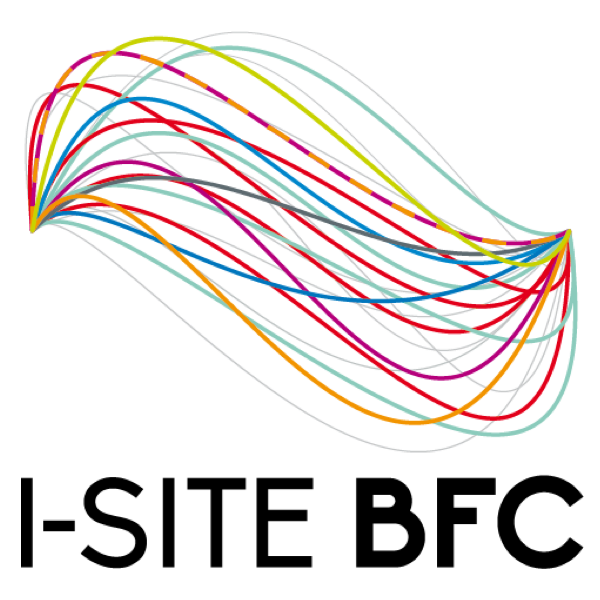
\includegraphics[width = 0.6\textwidth]{./logos/logo I-SITE BFC.png}}
			}
		child [grow = 90, level distance = 30em, concept color = color1!50]
			{
				node [level 1, text width = 18em, inner sep = -1em] (UB) {
\includegraphics[width = 0.6\textwidth]{./logos/logo UB.png}}
			};
	\begin{pgfonlayer}{background}
		\draw [densely dashed] 
			(Nom de projet)
				edge [color = color1!, line width = 1em] (UBFC)
				edge [color = color1!, line width = 1em] (UFC)
				edge [color = color1!, line width = 1em] (I-SITE BFC);
	\end{pgfonlayer}
\end{scope}



\begin{scope}
[
mindmap,
text = color0,
grow cyclic,
every node/.style =
{
	concept,
	concept color = color2!50,
	text = color0,
	execute at begin node = \hskip 0pt
},
root concept/.append style =
{
	concept color = color2,
	draw = color2!75,
	fill = color2!10,
	line width = 1em,
	text width = 20em,
	text = color0,
	font = \LARGE\scshape,
	inner sep = 0pt
},
level 1/.append style =
{
	concept color = color2,
	draw = color2!50,
	fill = color2!5,
	line width = 0.5em,
	text width = 18em,
	text = color0,
	font = \Large\bfseries,
	inner sep = 0pt
},
level 2/.append style =
{
	concept color = color2,
	draw = color2!50,
	fill = color2!5,
	line width = 0.5em,
	text width = 16em,
	text = color0,
	font = \large\bfseries,
	inner sep = 0pt
}
]

\node [root concept, text width = 20em, inner sep = -1em] (LLC)
at (15em, 35em)
{\LARGE{Pôle Lettres, \\Langues et \\Communication} \\\vspace{1em} \Huge{- LLC}}
	child [grow = -30, level distance = 30em, concept color = color2!50]
	{
		node [level 1, text width = 18em, inner sep = -1em] (LECLA) {
\includegraphics[width = 0.6\textwidth]{./logos/logo LECLA.png}}
	}
	child [grow = 150, level distance = 30em, concept color = color2!50]
	{
		node [level 1, text width = 18em, inner sep = -1em] (MSH Dijon) {
\includegraphics[width = 0.6\textwidth]{./logos/logo MSH Dijon.png}}
	}
	child [grow = -150, level distance = 30em, concept color = color2!50]
	{
		node [level 1, text width = 18em, inner sep = -1em] (MSHE) {
\includegraphics[width = 0.6\textwidth]{./logos/logo MSHE.png}}
	}
	child [grow = 30, level distance = 30em, concept color = color2!50]
	{
		node [level 1, text width = 18em, inner sep = -1em] (ELLIADD) {
\includegraphics[width = 0.6\textwidth]{./logos/logo ELLIADD.png}}
		child [grow = 0, level distance = 30em, concept color = color2!50]
		{
			node [level 2, text width = 16em, inner sep = -1em] (HULIN) {
\includegraphics[width = 0.9\textwidth]{./profiles/HULIN.png}}
		}
	};
\node[annotation, left,  concept color = color2, draw = color2!50, fill = color2!5, line width = 0.25em, text width = 17.5em, text = color0, font = \Large\bfseries, inner sep = 1em]
at (71em, 37.5em)
{\LARGE\bfseries{M. Thibaud HULIN \\\vspace{0.25em} Directeur de thèse}};
\begin{pgfonlayer}{background}
\draw [densely dashed] 
(Nom de projet)
	edge [color = color2!, line width = 1em] (LLC)
	edge [color = color2!, line width = 1em] (LECLA)
	edge [color = color2!, line width = 1em] (MSHE)
	edge [color = color2!, line width = 1em] (HULIN)
(MSHE)
	edge [color = color2!, line width = 1em] (UFC)
(MSH Dijon)
	edge [color = color2!, line width = 1em] (UB);
\end{pgfonlayer}
\end{scope}


\begin{scope}
[
mindmap,
text = color0,
grow cyclic,
every node/.style =
{
	concept,
	concept color = color3!50,
	text = color0,
	execute at begin node = \hskip 0pt
},
root concept/.append style =
{
	concept color = color3,
	draw = color3!75,
	fill = color3!10,
	line width = 1em,
	text width = 20em,
	text = color0,
	font = \LARGE\scshape,
	inner sep = 0pt
},
level 1/.append style =
{
	concept color = color3,
	draw = color3!50,
	fill = color3!5,
	line width = 0.5em,
	text width = 18em,
	text = color0,
	font = \Large\bfseries,
	inner sep = 0pt
},
level 2/.append style =
{
	concept color = color3,
	draw = color3!50,
	fill = color3!5,
	line width = 0.5em,
	text width = 16em,
	text = color0,
	font = \large\bfseries,
	inner sep = 0pt
}
]

\node [root concept, text width = 20em, inner sep = -1em] (HUMANE)
at (60em, 10em)
{\Huge{Projet \\HUMANE} \\\vspace{0.5em}\large{\og Humanités Numériques \\pour l'Éducation \fg}}
child [grow = 45, level distance = 30em, concept color = color3!50]
{
	node [level 1, text width = 18em, inner sep = -1em] (MENJS) {
\includegraphics[width = 0.6\textwidth]{./logos/logo MENJS.png}}
}
child [grow = -135, level distance = 30em, concept color = color3!50]
{
	node [level 1, text width = 18em, inner sep = -1em] (GIS 2IF) {
\includegraphics[width = 0.6\textwidth]{./logos/logo GIS 2IF.png}}
}
child [grow = -45, level distance = 30em, concept color = color3!50]
{
	node [level 1, text width = 18em, inner sep = -1em] (canope) {
\includegraphics[width = 0.6\textwidth]{./logos/logo canope.png}}
}
child [grow = 0, level distance = 30em, concept color = color3!50]
{
	node [level 1, text width = 18em, inner sep = -1em] (DRNE) {
\includegraphics[width = 0.6\textwidth]{./logos/logo DRNE.png}}
}
child [grow = -90, level distance = 30em, concept color = color3!50]
{
	node [level 1, text width = 18em, inner sep = -1em] (humanistica) {
\includegraphics[width = 0.6\textwidth]{./logos/logo humanistica.png}}
};
\begin{pgfonlayer}{background}
\draw [densely dashed] 
(HUMANE)
	edge [color = color3!, line width = 1em] (Nom de projet);
\end{pgfonlayer}
\end{scope}






\end{tikzpicture}

\end{document}
